\documentclass[]{article}
\usepackage{lmodern}
\usepackage{amssymb,amsmath}
\usepackage{ifxetex,ifluatex}
\usepackage{fixltx2e} % provides \textsubscript
\ifnum 0\ifxetex 1\fi\ifluatex 1\fi=0 % if pdftex
  \usepackage[T1]{fontenc}
  \usepackage[utf8]{inputenc}
\else % if luatex or xelatex
  \ifxetex
    \usepackage{mathspec}
  \else
    \usepackage{fontspec}
  \fi
  \defaultfontfeatures{Ligatures=TeX,Scale=MatchLowercase}
\fi
% use upquote if available, for straight quotes in verbatim environments
\IfFileExists{upquote.sty}{\usepackage{upquote}}{}
% use microtype if available
\IfFileExists{microtype.sty}{%
\usepackage{microtype}
\UseMicrotypeSet[protrusion]{basicmath} % disable protrusion for tt fonts
}{}
\usepackage[margin=1in]{geometry}
\usepackage{hyperref}
\hypersetup{unicode=true,
            pdftitle={Short PCA Vignette},
            pdfauthor={Aedin},
            pdfborder={0 0 0},
            breaklinks=true}
\urlstyle{same}  % don't use monospace font for urls
\usepackage{color}
\usepackage{fancyvrb}
\newcommand{\VerbBar}{|}
\newcommand{\VERB}{\Verb[commandchars=\\\{\}]}
\DefineVerbatimEnvironment{Highlighting}{Verbatim}{commandchars=\\\{\}}
% Add ',fontsize=\small' for more characters per line
\usepackage{framed}
\definecolor{shadecolor}{RGB}{248,248,248}
\newenvironment{Shaded}{\begin{snugshade}}{\end{snugshade}}
\newcommand{\KeywordTok}[1]{\textcolor[rgb]{0.13,0.29,0.53}{\textbf{#1}}}
\newcommand{\DataTypeTok}[1]{\textcolor[rgb]{0.13,0.29,0.53}{#1}}
\newcommand{\DecValTok}[1]{\textcolor[rgb]{0.00,0.00,0.81}{#1}}
\newcommand{\BaseNTok}[1]{\textcolor[rgb]{0.00,0.00,0.81}{#1}}
\newcommand{\FloatTok}[1]{\textcolor[rgb]{0.00,0.00,0.81}{#1}}
\newcommand{\ConstantTok}[1]{\textcolor[rgb]{0.00,0.00,0.00}{#1}}
\newcommand{\CharTok}[1]{\textcolor[rgb]{0.31,0.60,0.02}{#1}}
\newcommand{\SpecialCharTok}[1]{\textcolor[rgb]{0.00,0.00,0.00}{#1}}
\newcommand{\StringTok}[1]{\textcolor[rgb]{0.31,0.60,0.02}{#1}}
\newcommand{\VerbatimStringTok}[1]{\textcolor[rgb]{0.31,0.60,0.02}{#1}}
\newcommand{\SpecialStringTok}[1]{\textcolor[rgb]{0.31,0.60,0.02}{#1}}
\newcommand{\ImportTok}[1]{#1}
\newcommand{\CommentTok}[1]{\textcolor[rgb]{0.56,0.35,0.01}{\textit{#1}}}
\newcommand{\DocumentationTok}[1]{\textcolor[rgb]{0.56,0.35,0.01}{\textbf{\textit{#1}}}}
\newcommand{\AnnotationTok}[1]{\textcolor[rgb]{0.56,0.35,0.01}{\textbf{\textit{#1}}}}
\newcommand{\CommentVarTok}[1]{\textcolor[rgb]{0.56,0.35,0.01}{\textbf{\textit{#1}}}}
\newcommand{\OtherTok}[1]{\textcolor[rgb]{0.56,0.35,0.01}{#1}}
\newcommand{\FunctionTok}[1]{\textcolor[rgb]{0.00,0.00,0.00}{#1}}
\newcommand{\VariableTok}[1]{\textcolor[rgb]{0.00,0.00,0.00}{#1}}
\newcommand{\ControlFlowTok}[1]{\textcolor[rgb]{0.13,0.29,0.53}{\textbf{#1}}}
\newcommand{\OperatorTok}[1]{\textcolor[rgb]{0.81,0.36,0.00}{\textbf{#1}}}
\newcommand{\BuiltInTok}[1]{#1}
\newcommand{\ExtensionTok}[1]{#1}
\newcommand{\PreprocessorTok}[1]{\textcolor[rgb]{0.56,0.35,0.01}{\textit{#1}}}
\newcommand{\AttributeTok}[1]{\textcolor[rgb]{0.77,0.63,0.00}{#1}}
\newcommand{\RegionMarkerTok}[1]{#1}
\newcommand{\InformationTok}[1]{\textcolor[rgb]{0.56,0.35,0.01}{\textbf{\textit{#1}}}}
\newcommand{\WarningTok}[1]{\textcolor[rgb]{0.56,0.35,0.01}{\textbf{\textit{#1}}}}
\newcommand{\AlertTok}[1]{\textcolor[rgb]{0.94,0.16,0.16}{#1}}
\newcommand{\ErrorTok}[1]{\textcolor[rgb]{0.64,0.00,0.00}{\textbf{#1}}}
\newcommand{\NormalTok}[1]{#1}
\usepackage{longtable,booktabs}
\usepackage{graphicx,grffile}
\makeatletter
\def\maxwidth{\ifdim\Gin@nat@width>\linewidth\linewidth\else\Gin@nat@width\fi}
\def\maxheight{\ifdim\Gin@nat@height>\textheight\textheight\else\Gin@nat@height\fi}
\makeatother
% Scale images if necessary, so that they will not overflow the page
% margins by default, and it is still possible to overwrite the defaults
% using explicit options in \includegraphics[width, height, ...]{}
\setkeys{Gin}{width=\maxwidth,height=\maxheight,keepaspectratio}
\IfFileExists{parskip.sty}{%
\usepackage{parskip}
}{% else
\setlength{\parindent}{0pt}
\setlength{\parskip}{6pt plus 2pt minus 1pt}
}
\setlength{\emergencystretch}{3em}  % prevent overfull lines
\providecommand{\tightlist}{%
  \setlength{\itemsep}{0pt}\setlength{\parskip}{0pt}}
\setcounter{secnumdepth}{0}
% Redefines (sub)paragraphs to behave more like sections
\ifx\paragraph\undefined\else
\let\oldparagraph\paragraph
\renewcommand{\paragraph}[1]{\oldparagraph{#1}\mbox{}}
\fi
\ifx\subparagraph\undefined\else
\let\oldsubparagraph\subparagraph
\renewcommand{\subparagraph}[1]{\oldsubparagraph{#1}\mbox{}}
\fi

%%% Use protect on footnotes to avoid problems with footnotes in titles
\let\rmarkdownfootnote\footnote%
\def\footnote{\protect\rmarkdownfootnote}

%%% Change title format to be more compact
\usepackage{titling}

% Create subtitle command for use in maketitle
\providecommand{\subtitle}[1]{
  \posttitle{
    \begin{center}\large#1\end{center}
    }
}

\setlength{\droptitle}{-2em}

  \title{Short PCA Vignette}
    \pretitle{\vspace{\droptitle}\centering\huge}
  \posttitle{\par}
    \author{Aedin}
    \preauthor{\centering\large\emph}
  \postauthor{\par}
      \predate{\centering\large\emph}
  \postdate{\par}
    \date{May 1, 2018}


\begin{document}
\maketitle

\hypertarget{toy-data}{%
\section{Toy data}\label{toy-data}}

Create a cloud of points; two vectors, x,y of length 100. This example
dataset was included in Lior Patcher's blog
\url{https://liorpachter.wordpress.com/tag/least-squares/}

\begin{Shaded}
\begin{Highlighting}[]
 \KeywordTok{set.seed}\NormalTok{(}\DecValTok{2}\NormalTok{)             }\CommentTok{#sets the seed for random number generation.}
\NormalTok{ x <-}\StringTok{ }\DecValTok{1}\OperatorTok{:}\DecValTok{100}              \CommentTok{#creates a vector x with numbers from 1 to 100}
\NormalTok{ ex <-}\StringTok{ }\KeywordTok{rnorm}\NormalTok{(}\DecValTok{100}\NormalTok{, }\DecValTok{0}\NormalTok{, }\DecValTok{30}\NormalTok{) }\CommentTok{#100 normally distributed random numbers, mean=0, sd=30}
\NormalTok{ ey <-}\StringTok{ }\KeywordTok{rnorm}\NormalTok{(}\DecValTok{100}\NormalTok{, }\DecValTok{0}\NormalTok{, }\DecValTok{30}\NormalTok{) }\CommentTok{# 100 normally distributed random numbers, mean=0, sd=30}
\NormalTok{ y <-}\StringTok{ }\DecValTok{30} \OperatorTok{+}\StringTok{ }\DecValTok{2} \OperatorTok{*}\StringTok{ }\NormalTok{x         }\CommentTok{#sets y to be a vector that is a linear function of x}
\NormalTok{ x_obs <-}\StringTok{ }\NormalTok{x }\OperatorTok{+}\StringTok{ }\NormalTok{ex         }\CommentTok{#adds "noise" to x}
\NormalTok{ y_obs <-}\StringTok{ }\NormalTok{y }\OperatorTok{+}\StringTok{ }\NormalTok{ey         }\CommentTok{#adds "noise" to y}
 \KeywordTok{par}\NormalTok{(}\DataTypeTok{mfrow=}\KeywordTok{c}\NormalTok{(}\DecValTok{1}\NormalTok{,}\DecValTok{2}\NormalTok{))}
 \KeywordTok{hist}\NormalTok{(x_obs)}
 \KeywordTok{hist}\NormalTok{(y_obs)}
\end{Highlighting}
\end{Shaded}

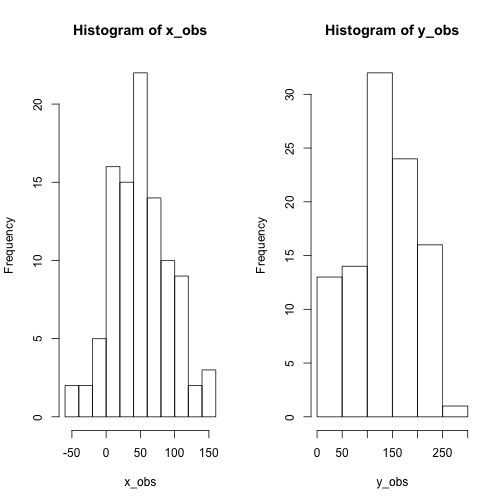
\includegraphics{PCA_files/figure-latex/unnamed-chunk-1-1.pdf}

Save both vectors in a matrix P

\begin{Shaded}
\begin{Highlighting}[]
\NormalTok{P <-}\StringTok{ }\KeywordTok{cbind}\NormalTok{(x_obs,y_obs) }\CommentTok{#places points in matrix}
\KeywordTok{summary}\NormalTok{(P)}
\end{Highlighting}
\end{Shaded}

\begin{verbatim}
##      x_obs            y_obs       
##  Min.   :-53.33   Min.   : 14.13  
##  1st Qu.: 21.44   1st Qu.: 97.22  
##  Median : 44.37   Median :134.91  
##  Mean   : 49.58   Mean   :131.88  
##  3rd Qu.: 77.91   3rd Qu.:174.29  
##  Max.   :155.78   Max.   :252.63
\end{verbatim}

Plot x,y. Show center (mean (x), mean(y)) on plot

\begin{Shaded}
\begin{Highlighting}[]
\KeywordTok{plot}\NormalTok{(P,}\DataTypeTok{asp=}\DecValTok{1}\NormalTok{,}\DataTypeTok{col=}\DecValTok{1}\NormalTok{) }\CommentTok{#plot points}
\KeywordTok{points}\NormalTok{(}\DataTypeTok{x=}\KeywordTok{mean}\NormalTok{(x_obs),}\DataTypeTok{y=}\KeywordTok{mean}\NormalTok{(y_obs),}\DataTypeTok{col=}\StringTok{"orange"}\NormalTok{, }\DataTypeTok{pch=}\DecValTok{19}\NormalTok{) }\CommentTok{#show center}
\end{Highlighting}
\end{Shaded}

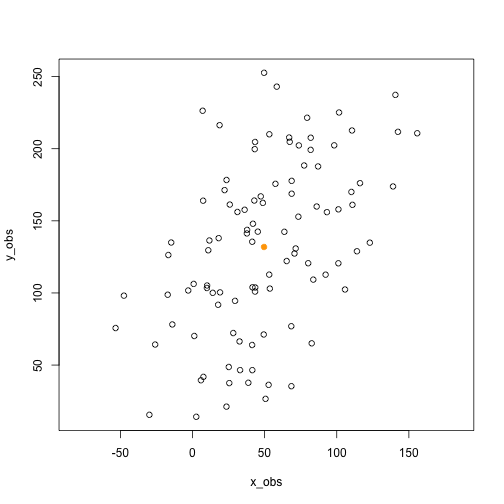
\includegraphics{PCA_files/figure-latex/unnamed-chunk-3-1.pdf}

\hypertarget{computing-via-svd-of-centered-covariance-matrix}{%
\section{Computing via svd of centered, covariance
matrix}\label{computing-via-svd-of-centered-covariance-matrix}}

PCA can be computed as a singular value decomposition of a column
centered matrix. Therefore we first processs the matrix.

\begin{Shaded}
\begin{Highlighting}[]
\NormalTok{M <-}\StringTok{ }\KeywordTok{cbind}\NormalTok{(x_obs}\OperatorTok{-}\KeywordTok{mean}\NormalTok{(x_obs),y_obs}\OperatorTok{-}\KeywordTok{mean}\NormalTok{(y_obs))}\CommentTok{#centered matrix}
\NormalTok{Mx<-}\KeywordTok{scale}\NormalTok{(P, }\DataTypeTok{scale=}\OtherTok{FALSE}\NormalTok{, }\DataTypeTok{center=}\OtherTok{TRUE}\NormalTok{)}
\KeywordTok{all.equal}\NormalTok{(M, Mx, }\DataTypeTok{check.attributes=}\OtherTok{FALSE}\NormalTok{)  }\CommentTok{# Is M equal to Mx, ignore col names}
\end{Highlighting}
\end{Shaded}

\begin{verbatim}
## [1] TRUE
\end{verbatim}

Singular value decomposition of M. The singular value decomposition of M
decomposes it into M=UDV\textsuperscript{t} where D is a diagonal matrix
and both U and V\textsuperscript{t} are orthogonal matrices.

\begin{Shaded}
\begin{Highlighting}[]
\NormalTok{ d <-}\StringTok{ }\KeywordTok{svd}\NormalTok{(M)}\OperatorTok{$}\NormalTok{d          }\CommentTok{#the singular values}
\NormalTok{ v <-}\StringTok{ }\KeywordTok{svd}\NormalTok{(M)}\OperatorTok{$}\NormalTok{v          }\CommentTok{#the right singular vectors}
\KeywordTok{svd}\NormalTok{(M)}\OperatorTok{$}\NormalTok{v}
\end{Highlighting}
\end{Shaded}

\begin{verbatim}
##           [,1]       [,2]
## [1,] 0.4527354 -0.8916449
## [2,] 0.8916449  0.4527354
\end{verbatim}

\hypertarget{eigenvector-eigenvalues-of-the-centered-covariance-matrix}{%
\section{Eigenvector, Eigenvalues of the centered, covariance
matrix}\label{eigenvector-eigenvalues-of-the-centered-covariance-matrix}}

The eigenvectors of the covariance matrix provide the principal axes,
and the eigenvalues quantify the fraction of variance explained in each
component.

\begin{Shaded}
\begin{Highlighting}[]
\NormalTok{MCov <-}\StringTok{ }\KeywordTok{cov}\NormalTok{(M)          }\CommentTok{#creates covariance matrix}
\NormalTok{eigenValues <-}\StringTok{ }\KeywordTok{eigen}\NormalTok{(MCov)}\OperatorTok{$}\NormalTok{values       }\CommentTok{#compute eigenvalues}
\NormalTok{eigenVectors <-}\StringTok{ }\KeywordTok{eigen}\NormalTok{(MCov)}\OperatorTok{$}\NormalTok{vectors     }\CommentTok{#compute eigenvectors}
\NormalTok{eigenValues}
\end{Highlighting}
\end{Shaded}

\begin{verbatim}
## [1] 4110.45 1189.45
\end{verbatim}

\begin{Shaded}
\begin{Highlighting}[]
\NormalTok{eigenVectors}
\end{Highlighting}
\end{Shaded}

\begin{verbatim}
##           [,1]       [,2]
## [1,] 0.4527354 -0.8916449
## [2,] 0.8916449  0.4527354
\end{verbatim}

The right singular vectors are the eigenvectors of
M\textsuperscript{t}M. Next I plot the principal axes:

\begin{Shaded}
\begin{Highlighting}[]
\KeywordTok{plot}\NormalTok{(P,}\DataTypeTok{asp=}\DecValTok{1}\NormalTok{,}\DataTypeTok{col=}\DecValTok{1}\NormalTok{) }\CommentTok{#plot points}
\KeywordTok{points}\NormalTok{(}\DataTypeTok{x=}\KeywordTok{mean}\NormalTok{(x_obs),}\DataTypeTok{y=}\KeywordTok{mean}\NormalTok{(y_obs),}\DataTypeTok{col=}\StringTok{"orange"}\NormalTok{, }\DataTypeTok{pch=}\DecValTok{19}\NormalTok{) }\CommentTok{#show center}
\KeywordTok{lines}\NormalTok{(x_obs,eigenVectors[}\DecValTok{2}\NormalTok{,}\DecValTok{1}\NormalTok{]}\OperatorTok{/}\NormalTok{eigenVectors[}\DecValTok{1}\NormalTok{,}\DecValTok{1}\NormalTok{]}\OperatorTok{*}\NormalTok{M[x]}\OperatorTok{+}\KeywordTok{mean}\NormalTok{(y_obs),}\DataTypeTok{col=}\DecValTok{8}\NormalTok{)}
\end{Highlighting}
\end{Shaded}

\includegraphics{PCA_files/figure-latex/unnamed-chunk-7-1.pdf}

This shows the first principal axis. Note that it passes through the
mean as expected. The ratio of the eigenvectors gives the slope of the
axis. Next

\begin{Shaded}
\begin{Highlighting}[]
\KeywordTok{plot}\NormalTok{(P,}\DataTypeTok{asp=}\DecValTok{1}\NormalTok{,}\DataTypeTok{col=}\DecValTok{1}\NormalTok{) }\CommentTok{#plot points}
\KeywordTok{points}\NormalTok{(}\DataTypeTok{x=}\KeywordTok{mean}\NormalTok{(x_obs),}\DataTypeTok{y=}\KeywordTok{mean}\NormalTok{(y_obs),}\DataTypeTok{col=}\StringTok{"orange"}\NormalTok{, }\DataTypeTok{pch=}\DecValTok{19}\NormalTok{) }\CommentTok{#show center}
\KeywordTok{lines}\NormalTok{(x_obs,eigenVectors[}\DecValTok{2}\NormalTok{,}\DecValTok{1}\NormalTok{]}\OperatorTok{/}\NormalTok{eigenVectors[}\DecValTok{1}\NormalTok{,}\DecValTok{1}\NormalTok{]}\OperatorTok{*}\NormalTok{M[x]}\OperatorTok{+}\KeywordTok{mean}\NormalTok{(y_obs),}\DataTypeTok{col=}\DecValTok{8}\NormalTok{)}
\KeywordTok{lines}\NormalTok{(x_obs,eigenVectors[}\DecValTok{2}\NormalTok{,}\DecValTok{2}\NormalTok{]}\OperatorTok{/}\NormalTok{eigenVectors[}\DecValTok{1}\NormalTok{,}\DecValTok{2}\NormalTok{]}\OperatorTok{*}\NormalTok{M[x]}\OperatorTok{+}\KeywordTok{mean}\NormalTok{(y_obs),}\DataTypeTok{col=}\DecValTok{8}\NormalTok{)}
\end{Highlighting}
\end{Shaded}

\includegraphics{PCA_files/figure-latex/unnamed-chunk-8-1.pdf} shows the
second principal axis, which is orthogonal to the first (recall that the
matrix V\textsuperscript{t} in the singular value decomposition is
orthogonal). This can be checked by noting that the second principal
axis is also

as the product of orthogonal slopes is -1. Next, I plot the projections
of the points onto the first principal component:

\begin{Shaded}
\begin{Highlighting}[]
\NormalTok{trans <-}\StringTok{ }\NormalTok{(M}\OperatorTok\NormalTok{v[,}\DecValTok{1}\NormalTok{])}\OperatorTok\NormalTok{v[,}\DecValTok{1}\NormalTok{] }\CommentTok{#compute projections of points}
\NormalTok{P_proj <-}\StringTok{ }\KeywordTok{scale}\NormalTok{(trans, }\DataTypeTok{center=}\OperatorTok{-}\KeywordTok{cbind}\NormalTok{(}\KeywordTok{mean}\NormalTok{(x_obs),}\KeywordTok{mean}\NormalTok{(y_obs)), }\DataTypeTok{scale=}\OtherTok{FALSE}\NormalTok{) }

\KeywordTok{plot}\NormalTok{(P,}\DataTypeTok{asp=}\DecValTok{1}\NormalTok{,}\DataTypeTok{col=}\DecValTok{1}\NormalTok{) }\CommentTok{#plot points}
\KeywordTok{lines}\NormalTok{(x_obs,eigenVectors[}\DecValTok{2}\NormalTok{,}\DecValTok{1}\NormalTok{]}\OperatorTok{/}\NormalTok{eigenVectors[}\DecValTok{1}\NormalTok{,}\DecValTok{1}\NormalTok{]}\OperatorTok{*}\NormalTok{M[x]}\OperatorTok{+}\KeywordTok{mean}\NormalTok{(y_obs),}\DataTypeTok{col=}\DecValTok{8}\NormalTok{)}
\KeywordTok{lines}\NormalTok{(x_obs,eigenVectors[}\DecValTok{2}\NormalTok{,}\DecValTok{2}\NormalTok{]}\OperatorTok{/}\NormalTok{eigenVectors[}\DecValTok{1}\NormalTok{,}\DecValTok{2}\NormalTok{]}\OperatorTok{*}\NormalTok{M[x]}\OperatorTok{+}\KeywordTok{mean}\NormalTok{(y_obs),}\DataTypeTok{col=}\DecValTok{8}\NormalTok{)}
\CommentTok{#points(P_proj, col=4,pch=19,cex=0.5) #plot projections}
\KeywordTok{segments}\NormalTok{(x_obs,y_obs,P_proj[,}\DecValTok{1}\NormalTok{],P_proj[,}\DecValTok{2}\NormalTok{],}\DataTypeTok{col=}\DecValTok{4}\NormalTok{,}\DataTypeTok{lty=}\DecValTok{2}\NormalTok{) }\CommentTok{#connect to points}
\end{Highlighting}
\end{Shaded}

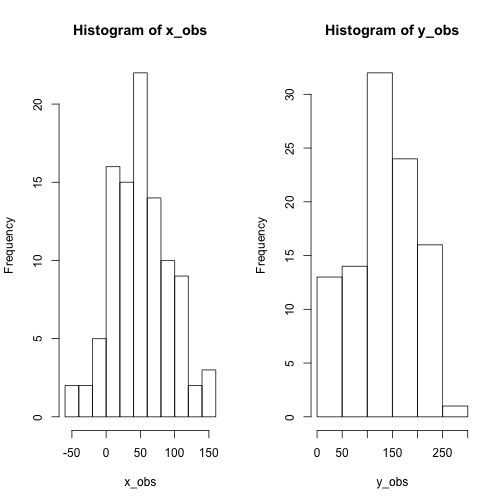
\includegraphics{PCA_files/figure-latex/unnamed-chunk-9-1.pdf}

\hypertarget{pca-in-r}{%
\section{PCA in R}\label{pca-in-r}}

In R, there are several functions from different packages that allow us
to perform PCA. These include;

\begin{itemize}
\tightlist
\item
  prcomp() (stats)
\item
  princomp() (stats)
\item
  PCA() (FactoMineR)
\item
  dudi.pca() (ade4)
\end{itemize}

We will demonstrate some of these and explore these using exploR

\hypertarget{equivalents-across-methods}{%
\section{Equivalents across methods}\label{equivalents-across-methods}}

Give an input matrix P and result res

\begin{longtable}[]{@{}llll@{}}
\toprule
Function & loadings & scores & plot\tabularnewline
\midrule
\endhead
prcomp(P, center=TRUE, scale=TRUE) & res\$rotation & res\$x &
biplot(res)\tabularnewline
princomp(P, cor=TRUE) & res\$loadings & res\$scores &
biplot(res)\tabularnewline
PCA(P) & res\$svd\$V & res\$ind\$coord & plot(res)\tabularnewline
dudi.pca(P, center=TRUE, scale=TRUE) & res\$c1 & res\$li &
scatter(res)\tabularnewline
\bottomrule
\end{longtable}

With ade4::dudi.pca and prcomp the default is center = TRUE, scale =
TRUE.But with princomp, cor=FALSE by default.

\hypertarget{svd}{%
\subsection{svd}\label{svd}}

To get the equivalent result using svd or eigen above, repeat the code
above but scale and center the data scale(P, center=TRUE, scale=TRUE).

\begin{Shaded}
\begin{Highlighting}[]
\KeywordTok{svd}\NormalTok{(}\KeywordTok{scale}\NormalTok{(P))}\OperatorTok{$}\NormalTok{v}
\end{Highlighting}
\end{Shaded}

\begin{verbatim}
##           [,1]       [,2]
## [1,] 0.7071068 -0.7071068
## [2,] 0.7071068  0.7071068
\end{verbatim}

\hypertarget{prcomp}{%
\subsection{prcomp}\label{prcomp}}

First stats::prcomp. The eigenvector are stored in \$rotation

\begin{Shaded}
\begin{Highlighting}[]
\NormalTok{p1<-}\StringTok{ }\KeywordTok{prcomp}\NormalTok{(P, }\DataTypeTok{scale =} \OtherTok{TRUE}\NormalTok{)}
\NormalTok{p1}
\end{Highlighting}
\end{Shaded}

\begin{verbatim}
## Standard deviations (1, .., p=2):
## [1] 1.212661 0.727635
## 
## Rotation (n x k) = (2 x 2):
##             PC1        PC2
## x_obs 0.7071068 -0.7071068
## y_obs 0.7071068  0.7071068
\end{verbatim}

\begin{Shaded}
\begin{Highlighting}[]
\KeywordTok{summary}\NormalTok{(p1)}
\end{Highlighting}
\end{Shaded}

\begin{verbatim}
## Importance of components:
##                           PC1    PC2
## Standard deviation     1.2127 0.7276
## Proportion of Variance 0.7353 0.2647
## Cumulative Proportion  0.7353 1.0000
\end{verbatim}

\begin{Shaded}
\begin{Highlighting}[]
\CommentTok{# This can be calculated as;}
\NormalTok{eigs=}\StringTok{ }\NormalTok{p1}\OperatorTok{$}\NormalTok{sdev}\OperatorTok{^}\DecValTok{2}
\NormalTok{eigSum=}\StringTok{ }\KeywordTok{rbind}\NormalTok{(}
  \DataTypeTok{SD =} \KeywordTok{sqrt}\NormalTok{(eigs),}
  \DataTypeTok{Proportion =}\NormalTok{ eigs}\OperatorTok{/}\KeywordTok{sum}\NormalTok{(eigs),}
  \DataTypeTok{Cumulative =} \KeywordTok{cumsum}\NormalTok{(eigs)}\OperatorTok{/}\KeywordTok{sum}\NormalTok{(eigs))}

\NormalTok{eigSum}
\end{Highlighting}
\end{Shaded}

\begin{verbatim}
##                 [,1]      [,2]
## SD         1.2126612 0.7276350
## Proportion 0.7352736 0.2647264
## Cumulative 0.7352736 1.0000000
\end{verbatim}

\hypertarget{princomp}{%
\section{princomp}\label{princomp}}

\begin{Shaded}
\begin{Highlighting}[]
\NormalTok{p2<-stats}\OperatorTok{::}\KeywordTok{princomp}\NormalTok{(P)}

\CommentTok{# sqrt of eigenvalues}
\NormalTok{p2}\OperatorTok{$}\NormalTok{sdev}
\end{Highlighting}
\end{Shaded}

\begin{verbatim}
##   Comp.1   Comp.2 
## 63.79142 34.31553
\end{verbatim}

\begin{Shaded}
\begin{Highlighting}[]
\CommentTok{# eigenvectors}
\NormalTok{p2}\OperatorTok{$}\NormalTok{loadings}
\end{Highlighting}
\end{Shaded}

\begin{verbatim}
## 
## Loadings:
##       Comp.1 Comp.2
## x_obs  0.453  0.892
## y_obs  0.892 -0.453
## 
##                Comp.1 Comp.2
## SS loadings       1.0    1.0
## Proportion Var    0.5    0.5
## Cumulative Var    0.5    1.0
\end{verbatim}

\hypertarget{factominer}{%
\subsection{FactoMineR}\label{factominer}}

FactoMineR::PCA calls svd to compute the PCA

\begin{Shaded}
\begin{Highlighting}[]
\NormalTok{p3<-FactoMineR}\OperatorTok{::}\KeywordTok{PCA}\NormalTok{(P)}
\end{Highlighting}
\end{Shaded}

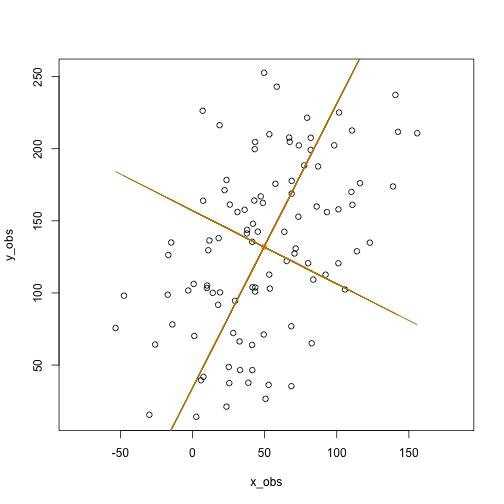
\includegraphics{PCA_files/figure-latex/unnamed-chunk-13-1.pdf}
\includegraphics{PCA_files/figure-latex/unnamed-chunk-13-2.pdf}

\begin{Shaded}
\begin{Highlighting}[]
\NormalTok{p3}\OperatorTok{$}\NormalTok{eig}
\end{Highlighting}
\end{Shaded}

\begin{verbatim}
##        eigenvalue percentage of variance cumulative percentage of variance
## comp 1  1.4705472               73.52736                          73.52736
## comp 2  0.5294528               26.47264                         100.00000
\end{verbatim}

\begin{Shaded}
\begin{Highlighting}[]
\NormalTok{p3}\OperatorTok{$}\NormalTok{var}\OperatorTok{$}\NormalTok{coord  }\CommentTok{# correlations between variables and PCs}
\end{Highlighting}
\end{Shaded}

\begin{verbatim}
##          Dim.1      Dim.2
## x_obs 0.857481  0.5145157
## y_obs 0.857481 -0.5145157
\end{verbatim}

\hypertarget{ade4dudi.pca}{%
\subsection{ADE4::dudi.pca}\label{ade4dudi.pca}}

First ade4::dudi.pca scales the data and stores the scaled data in
\$tab. In PCA this will be almost equivalent to scale. However there is
a minor difference (see
\url{https://pbil.univ-lyon1.fr/R/pdf/course2.pdf}). ade4 usees the
duality diagram framework for computing pca and other matrix
factorizations (so it provides lw and cw which are the row and columns
weights). See Cruz and Holmes 2011 for a wonderful tutorial on the
duality diagram framework
\url{https://www.ncbi.nlm.nih.gov/pmc/articles/PMC3265363/}

\begin{Shaded}
\begin{Highlighting}[]
\NormalTok{p4<-ade4}\OperatorTok{::}\KeywordTok{dudi.pca}\NormalTok{(P, }\DataTypeTok{scannf =} \OtherTok{FALSE}\NormalTok{, }\DataTypeTok{nf=}\DecValTok{2}\NormalTok{)  }\CommentTok{# save 2 axis by default,}
\KeywordTok{head}\NormalTok{(p4}\OperatorTok{$}\NormalTok{tab)  }\CommentTok{# centered/scaled data. }
\end{Highlighting}
\end{Shaded}

\begin{verbatim}
##         x_obs      y_obs
## 1 -1.79410466 -1.1472082
## 2 -0.99902168 -1.5273772
## 3  0.02510543 -1.7859484
## 4 -1.88926469 -1.9735368
## 5 -1.11674143 -1.9968913
## 6 -0.94133545 -0.4822568
\end{verbatim}

\begin{Shaded}
\begin{Highlighting}[]
\KeywordTok{head}\NormalTok{(}\KeywordTok{scale}\NormalTok{(P))}
\end{Highlighting}
\end{Shaded}

\begin{verbatim}
##            x_obs      y_obs
## [1,] -1.78511160 -1.1414577
## [2,] -0.99401402 -1.5197211
## [3,]  0.02497959 -1.7769963
## [4,] -1.87979464 -1.9636443
## [5,] -1.11114369 -1.9868817
## [6,] -0.93661695 -0.4798394
\end{verbatim}

The values used for centering are stored in cent, it is a the colMeans.
norm provides the sd of the columns

\begin{Shaded}
\begin{Highlighting}[]
\NormalTok{p4}\OperatorTok{$}\NormalTok{cent }\OperatorTok{==}\StringTok{ }\KeywordTok{colMeans}\NormalTok{(P)}
\end{Highlighting}
\end{Shaded}

\begin{verbatim}
## x_obs y_obs 
##  TRUE  TRUE
\end{verbatim}

\begin{Shaded}
\begin{Highlighting}[]
\NormalTok{sd.n <-}\StringTok{ }\ControlFlowTok{function}\NormalTok{(x) }\KeywordTok{sqrt}\NormalTok{(}\KeywordTok{var}\NormalTok{(x) }\OperatorTok{*}\StringTok{ }\NormalTok{(}\KeywordTok{length}\NormalTok{(x) }\OperatorTok{-}\StringTok{ }\DecValTok{1}\NormalTok{)}\OperatorTok{/}\KeywordTok{length}\NormalTok{(x))}
\KeywordTok{identical}\NormalTok{(p4}\OperatorTok{$}\NormalTok{norm,}\KeywordTok{apply}\NormalTok{(P, }\DecValTok{2}\NormalTok{, sd.n))}
\end{Highlighting}
\end{Shaded}

\begin{verbatim}
## [1] TRUE
\end{verbatim}

The summary printout is equivalent to P3
(p3\(eig) above. The eigenvales are stored in p4\)eig.

\begin{Shaded}
\begin{Highlighting}[]
\KeywordTok{summary}\NormalTok{(p4)}
\end{Highlighting}
\end{Shaded}

\begin{verbatim}
## Class: pca dudi
## Call: ade4::dudi.pca(df = P, scannf = FALSE, nf = 2)
## 
## Total inertia: 2
## 
## Eigenvalues:
##     Ax1     Ax2 
##  1.4705  0.5295 
## 
## Projected inertia (%):
##     Ax1     Ax2 
##   73.53   26.47 
## 
## Cumulative projected inertia (%):
##     Ax1   Ax1:2 
##   73.53  100.00
\end{verbatim}

\begin{Shaded}
\begin{Highlighting}[]
\NormalTok{p4}\OperatorTok{$}\NormalTok{eig}
\end{Highlighting}
\end{Shaded}

\begin{verbatim}
## [1] 1.4705472 0.5294528
\end{verbatim}

\begin{Shaded}
\begin{Highlighting}[]
\NormalTok{p4}\OperatorTok{$}\NormalTok{c1}
\end{Highlighting}
\end{Shaded}

\begin{verbatim}
##             CS1        CS2
## x_obs 0.7071068 -0.7071068
## y_obs 0.7071068  0.7071068
\end{verbatim}

\begin{Shaded}
\begin{Highlighting}[]
\NormalTok{p4}\OperatorTok{$}\NormalTok{co}
\end{Highlighting}
\end{Shaded}

\begin{verbatim}
##          Comp1      Comp2
## x_obs 0.857481 -0.5145157
## y_obs 0.857481  0.5145157
\end{verbatim}

The cumulative \% of variance explained by each component ;

\begin{Shaded}
\begin{Highlighting}[]
\NormalTok{(k <-}\StringTok{ }\DecValTok{100} \OperatorTok{*}\StringTok{ }\NormalTok{p4}\OperatorTok{$}\NormalTok{eig}\OperatorTok{/}\KeywordTok{sum}\NormalTok{(p4}\OperatorTok{$}\NormalTok{eig))}
\end{Highlighting}
\end{Shaded}

\begin{verbatim}
## [1] 73.52736 26.47264
\end{verbatim}

\begin{Shaded}
\begin{Highlighting}[]
\KeywordTok{cumsum}\NormalTok{(k)}
\end{Highlighting}
\end{Shaded}

\begin{verbatim}
## [1]  73.52736 100.00000
\end{verbatim}

nf is an integer giving the number of axes kept. nf will always be lower
that the number of row or columns of the matrix -1.

\begin{Shaded}
\begin{Highlighting}[]
\NormalTok{p4}\OperatorTok{$}\NormalTok{nf}
\end{Highlighting}
\end{Shaded}

\begin{verbatim}
## [1] 2
\end{verbatim}

c1 gives the variables' coordinates, normed to 1. It is also called the
coefficients of the combination or the loadings of variables. Equally
the outpur matrix l1 gives the individuals' coordinates, normed to 1. It
is also called the loadings of individuals.

\begin{Shaded}
\begin{Highlighting}[]
\NormalTok{p4}\OperatorTok{$}\NormalTok{c1}
\end{Highlighting}
\end{Shaded}

\begin{verbatim}
##             CS1        CS2
## x_obs 0.7071068 -0.7071068
## y_obs 0.7071068  0.7071068
\end{verbatim}

\begin{Shaded}
\begin{Highlighting}[]
\KeywordTok{sum}\NormalTok{(p4}\OperatorTok{$}\NormalTok{cw }\OperatorTok{*}\StringTok{ }\NormalTok{p4}\OperatorTok{$}\NormalTok{c1}\OperatorTok{$}\NormalTok{CS1}\OperatorTok{^}\DecValTok{2}\NormalTok{)}
\end{Highlighting}
\end{Shaded}

\begin{verbatim}
## [1] 1
\end{verbatim}

co gives the variables' coordinates, normed to the square root of the
eigenvalues.

\begin{Shaded}
\begin{Highlighting}[]
\NormalTok{p4}\OperatorTok{$}\NormalTok{co}
\end{Highlighting}
\end{Shaded}

\begin{verbatim}
##          Comp1      Comp2
## x_obs 0.857481 -0.5145157
## y_obs 0.857481  0.5145157
\end{verbatim}

\begin{Shaded}
\begin{Highlighting}[]
\KeywordTok{sum}\NormalTok{(p4}\OperatorTok{$}\NormalTok{cw }\OperatorTok{*}\StringTok{ }\NormalTok{p4}\OperatorTok{$}\NormalTok{co}\OperatorTok{$}\NormalTok{Comp1}\OperatorTok{^}\DecValTok{2}\NormalTok{)}
\end{Highlighting}
\end{Shaded}

\begin{verbatim}
## [1] 1.470547
\end{verbatim}

The link between c1 and co is defined by:

\begin{Shaded}
\begin{Highlighting}[]
\NormalTok{p4}\OperatorTok{$}\NormalTok{c1}\OperatorTok{$}\NormalTok{CS1 }\OperatorTok{*}\StringTok{ }\KeywordTok{sqrt}\NormalTok{(p4}\OperatorTok{$}\NormalTok{eig[}\DecValTok{1}\NormalTok{])}
\end{Highlighting}
\end{Shaded}

\begin{verbatim}
## [1] 0.857481 0.857481
\end{verbatim}

\hypertarget{visualization-and-exploration-of-results}{%
\section{Visualization and Exploration of
results}\label{visualization-and-exploration-of-results}}

The github package \url{https://github.com/juba/explor} is useful for
exploring data. It includes plotting functions for many packages
including ade4, FactoMineR and baseR functions prcomp and princomp;

For now on, it is usable the following types of analyses :

\begin{longtable}[]{@{}llll@{}}
\toprule
\begin{minipage}[b]{0.17\columnwidth}\raggedright
Analysis\strut
\end{minipage} & \begin{minipage}[b]{0.17\columnwidth}\raggedright
Function\strut
\end{minipage} & \begin{minipage}[b]{0.14\columnwidth}\raggedright
Package\strut
\end{minipage} & \begin{minipage}[b]{0.11\columnwidth}\raggedright
Notes\strut
\end{minipage}\tabularnewline
\midrule
\endhead
\begin{minipage}[t]{0.17\columnwidth}\raggedright
Principal Component Analysis\strut
\end{minipage} & \begin{minipage}[t]{0.17\columnwidth}\raggedright
PCA\strut
\end{minipage} & \begin{minipage}[t]{0.14\columnwidth}\raggedright
\href{http://factominer.free.fr/}{FactoMineR}\strut
\end{minipage} & \begin{minipage}[t]{0.11\columnwidth}\raggedright
-\strut
\end{minipage}\tabularnewline
\begin{minipage}[t]{0.17\columnwidth}\raggedright
Correspondance Analysis\strut
\end{minipage} & \begin{minipage}[t]{0.17\columnwidth}\raggedright
CA\strut
\end{minipage} & \begin{minipage}[t]{0.14\columnwidth}\raggedright
\href{http://factominer.free.fr/}{FactoMineR}\strut
\end{minipage} & \begin{minipage}[t]{0.11\columnwidth}\raggedright
-\strut
\end{minipage}\tabularnewline
\begin{minipage}[t]{0.17\columnwidth}\raggedright
Multiple Correspondence Analysis\strut
\end{minipage} & \begin{minipage}[t]{0.17\columnwidth}\raggedright
MCA\strut
\end{minipage} & \begin{minipage}[t]{0.14\columnwidth}\raggedright
\href{http://factominer.free.fr/}{FactoMineR}\strut
\end{minipage} & \begin{minipage}[t]{0.11\columnwidth}\raggedright
-\strut
\end{minipage}\tabularnewline
\begin{minipage}[t]{0.17\columnwidth}\raggedright
Principal Component Analysis\strut
\end{minipage} & \begin{minipage}[t]{0.17\columnwidth}\raggedright
dudi.pca\strut
\end{minipage} & \begin{minipage}[t]{0.14\columnwidth}\raggedright
\href{https://cran.r-project.org/package=ade4}{ade4}\strut
\end{minipage} & \begin{minipage}[t]{0.11\columnwidth}\raggedright
Qualitative supplementary variables are ignored\strut
\end{minipage}\tabularnewline
\begin{minipage}[t]{0.17\columnwidth}\raggedright
Correspondance Analysis\strut
\end{minipage} & \begin{minipage}[t]{0.17\columnwidth}\raggedright
dudi.coa\strut
\end{minipage} & \begin{minipage}[t]{0.14\columnwidth}\raggedright
\href{https://cran.r-project.org/package=ade4}{ade4}\strut
\end{minipage} & \begin{minipage}[t]{0.11\columnwidth}\raggedright
-\strut
\end{minipage}\tabularnewline
\begin{minipage}[t]{0.17\columnwidth}\raggedright
Multiple Correspondence Analysis\strut
\end{minipage} & \begin{minipage}[t]{0.17\columnwidth}\raggedright
dudi.acm\strut
\end{minipage} & \begin{minipage}[t]{0.14\columnwidth}\raggedright
\href{https://cran.r-project.org/package=ade4}{ade4}\strut
\end{minipage} & \begin{minipage}[t]{0.11\columnwidth}\raggedright
Quantitative supplementary variables are ignored\strut
\end{minipage}\tabularnewline
\begin{minipage}[t]{0.17\columnwidth}\raggedright
Specific Multiple Correspondance Analysis\strut
\end{minipage} & \begin{minipage}[t]{0.17\columnwidth}\raggedright
speMCA\strut
\end{minipage} & \begin{minipage}[t]{0.14\columnwidth}\raggedright
\href{https://cran.r-project.org/package=GDAtools}{GDAtools}\strut
\end{minipage} & \begin{minipage}[t]{0.11\columnwidth}\raggedright
Supplementary variables are not supported\strut
\end{minipage}\tabularnewline
\begin{minipage}[t]{0.17\columnwidth}\raggedright
Multiple Correspondance Analysis\strut
\end{minipage} & \begin{minipage}[t]{0.17\columnwidth}\raggedright
mca\strut
\end{minipage} & \begin{minipage}[t]{0.14\columnwidth}\raggedright
\href{https://cran.r-project.org/package=MASS}{MASS}\strut
\end{minipage} & \begin{minipage}[t]{0.11\columnwidth}\raggedright
Quantitative supplementary variables are not supported\strut
\end{minipage}\tabularnewline
\begin{minipage}[t]{0.17\columnwidth}\raggedright
Principal Component Analysis\strut
\end{minipage} & \begin{minipage}[t]{0.17\columnwidth}\raggedright
princomp\strut
\end{minipage} & \begin{minipage}[t]{0.14\columnwidth}\raggedright
stats\strut
\end{minipage} & \begin{minipage}[t]{0.11\columnwidth}\raggedright
Supplementary variables are ignored\strut
\end{minipage}\tabularnewline
\begin{minipage}[t]{0.17\columnwidth}\raggedright
Principal Component Analysis\strut
\end{minipage} & \begin{minipage}[t]{0.17\columnwidth}\raggedright
prcomp\strut
\end{minipage} & \begin{minipage}[t]{0.14\columnwidth}\raggedright
stats\strut
\end{minipage} & \begin{minipage}[t]{0.11\columnwidth}\raggedright
Supplementary variables are ignored\strut
\end{minipage}\tabularnewline
\bottomrule
\end{longtable}

\begin{Shaded}
\begin{Highlighting}[]
\ControlFlowTok{if}\NormalTok{(}\OperatorTok{!}\StringTok{"explor"} \OperatorTok\StringTok{ }\KeywordTok{rownames}\NormalTok{(}\KeywordTok{installed.packages}\NormalTok{()))    devtools}\OperatorTok{::}\KeywordTok{install_github}\NormalTok{(}\StringTok{"juba/explor"}\NormalTok{)}

\ControlFlowTok{if}\NormalTok{(}\OperatorTok{!}\StringTok{"scatterD3"} \OperatorTok\StringTok{ }\KeywordTok{rownames}\NormalTok{(}\KeywordTok{installed.packages}\NormalTok{())) }
\NormalTok{devtools}\OperatorTok{::}\KeywordTok{install_github}\NormalTok{(}\StringTok{"juba/scatterD3"}\NormalTok{)}
\end{Highlighting}
\end{Shaded}

\begin{Shaded}
\begin{Highlighting}[]
\KeywordTok{require}\NormalTok{(explor)}
\NormalTok{explor}\OperatorTok{::}\KeywordTok{explor}\NormalTok{(p4)}
\end{Highlighting}
\end{Shaded}

\begin{Shaded}
\begin{Highlighting}[]
\KeywordTok{data}\NormalTok{(children)}
\NormalTok{res.ca <-}\StringTok{ }\KeywordTok{CA}\NormalTok{(children, }\DataTypeTok{row.sup =} \DecValTok{15}\OperatorTok{:}\DecValTok{18}\NormalTok{, }\DataTypeTok{col.sup =} \DecValTok{6}\OperatorTok{:}\DecValTok{8}\NormalTok{)}
\KeywordTok{explor}\NormalTok{(res.ca)}
\end{Highlighting}
\end{Shaded}


\end{document}
